% Source PDF page 501 (printed p. 487)
停止准则。可以将牛顿减量与量 $f(x)-\inf_y\widehat f(y)$ 联系起来，其中 $\widehat f$ 为 $f$ 在 $x$ 的二阶近似：
\[
f(x)-\inf_y\widehat f(y)=f(x)-\widehat f(x+\Delta x_{\mathrm{nt}})
=\tfrac12\lambda(x)^2.
\]
因此，$\lambda^2/2$ 是基于 $f$ 在 $x$ 的二次近似，对 $f(x)-p^\star$ 作出的估计。

还可把牛顿减量写为
\begin{equation}
\lambda(x)=\bigl(\Delta x_{\mathrm{nt}}^\T\nabla^2f(x)\Delta x_{\mathrm{nt}}\bigr)^{1/2}.\tag{9.29}
\end{equation}
这说明 $\lambda$ 是Hessian定义的二次范数下牛顿步的范数，即范数
\[
\norm u_{\nabla^2f(x)}=(u^\T\nabla^2f(x)u)^{1/2}.
\]
牛顿减量也出现在回溯线搜索中，因为
\begin{equation}
\nabla f(x)^\T\Delta x_{\mathrm{nt}}=-\lambda(x)^2.\tag{9.30}
\end{equation}
它就是回溯线搜索使用的常数，并可解释为 $f$ 在 $x$ 处沿牛顿步的方向导数：
\[
-\lambda(x)^2=\nabla f(x)^\T\Delta x_{\mathrm{nt}}
=\left.\frac{\mathrm d}{\mathrm dt}f(x+\Delta x_{\mathrm{nt}}t)\right|_{t=0}.
\]

最后，牛顿减量与牛顿步一样具有仿射不变性。即当 $T$ 非奇异时，$\overline f(y)=f(Ty)$ 在 $y$ 的牛顿减量，与 $f$ 在 $x=Ty$ 的牛顿减量相同。

\subsection{牛顿法}
下面概述的牛顿法有时称为\emph{阻尼牛顿法}或\emph{保护牛顿法}，以区别于采用固定步长 $t=1$ 的\emph{纯牛顿法}。

\begin{origalgorithm}{9.5}
\emph{牛顿法。}

给定初始点 $x\in\dom f$，容差 $\epsilon>0$。

重复：
\begin{enumerate}
\item \emph{计算牛顿步与减量。}
\[
\Delta x_{\mathrm{nt}}:=-\nabla^2f(x)^{-1}\nabla f(x),\qquad
\lambda^2:=\nabla f(x)^\T\nabla^2f(x)^{-1}\nabla f(x).
\]
\item \emph{停止准则。}若 $\lambda^2/2\le\epsilon$，退出。
\item \emph{线搜索。}用回溯线搜索选择步长 $t$。
\item \emph{更新。}$x:=x+t\Delta x_{\mathrm{nt}}$。
\end{enumerate}
\end{origalgorithm}

它基本就是§9.2的一般下降方法，搜索方向取牛顿步。唯一差别很小：在计算搜索方向后检查停止准则，而非在更新后检查。

% Source PDF page 502 (printed p. 488)
\subsection{收敛分析}
仍假设 $f$ 二阶连续可微，且以常数 $m$ 强凸，即对 $x\in S$，$\nabla^2f(x)\succeq mI$。已知这还蕴含存在 $M>0$，使所有 $x\in S$ 满足 $\nabla^2f(x)\preceq MI$。

此外，假设 $f$ 的Hessian在 $S$ 上Lipschitz连续，常数为 $L$，即所有 $x,y\in S$ 满足
\begin{equation}
\norm{\nabla^2f(x)-\nabla^2f(y)}_2\le L\norm{x-y}_2.\tag{9.31}
\end{equation}
系数 $L$ 可理解为 $f$ 三阶导数的界；二次函数可取 $L=0$。更一般地，$L$ 衡量二次模型对 $f$ 的近似程度，因此可预期它对牛顿法性能起关键作用。直觉表明，若函数的二次模型变化缓慢（即 $L$ 小），牛顿法会非常有效。

\subsubsection*{收敛证明的思想与框架}
先给出证明的思想、框架和主要结论，再给出细节。将证明存在数 $\eta,\gamma$，其中 $0<\eta\le m^2/L$、$\gamma>0$，满足：
\begin{itemize}
\item 若 $\norm{\nabla f(x^{(k)})}_2\ge\eta$，则
\begin{equation}
f(x^{(k+1)})-f(x^{(k)})\le-\gamma.\tag{9.32}
\end{equation}
\item 若 $\norm{\nabla f(x^{(k)})}_2<\eta$，则回溯线搜索选择 $t^{(k)}=1$，且
\begin{equation}
\frac L{2m^2}\norm{\nabla f(x^{(k+1)})}_2
\le\left(\frac L{2m^2}\norm{\nabla f(x^{(k)})}_2\right)^2.\tag{9.33}
\end{equation}
\end{itemize}
分析第二个条件的含义。设它在第 $k$ 次迭代满足，即 $\norm{\nabla f(x^{(k)})}_2<\eta$。由于 $\eta\le m^2/L$，有 $\norm{\nabla f(x^{(k+1)})}_2<\eta$，所以第 $k+1$ 次也满足。递归下去，一旦第二个条件成立，所有后续迭代都成立，即对所有 $l\ge k$，$\norm{\nabla f(x^{(l)})}_2<\eta$。因此，对所有 $l\ge k$，算法都采用完整牛顿步 $t=1$，且
\begin{equation}
\frac L{2m^2}\norm{\nabla f(x^{(l+1)})}_2
\le\left(\frac L{2m^2}\norm{\nabla f(x^{(l)})}_2\right)^2.\tag{9.34}
\end{equation}
递归应用可知，对于 $l\ge k$，
\[
\frac L{2m^2}\norm{\nabla f(x^{(l)})}_2
\le\left(\frac L{2m^2}\norm{\nabla f(x^{(k)})}_2\right)^{2^{l-k}}
\le\left(\frac12\right)^{2^{l-k}},
\]
进而
\begin{equation}
f(x^{(l)})-p^\star\le\frac1{2m}\norm{\nabla f(x^{(l)})}_2^2
\le\frac{2m^3}{L^2}\left(\frac12\right)^{2^{l-k+1}}.\tag{9.35}
\end{equation}

% Source PDF page 503 (printed p. 489)
最后的不等式说明，一旦满足第二个条件，收敛就极快。这一现象称为\emph{二次收敛}。粗略地说，（9.35）意味着迭代足够多次后，每次迭代使正确数字位数加倍。

牛顿法迭代自然分为两个阶段。条件 $\norm{\nabla f(x)}_2\le\eta$ 成立后进入第二阶段，称为\emph{二次收敛阶段}。第一阶段称为\emph{阻尼牛顿阶段}，因为算法可能选择 $t<1$。二次收敛阶段也称\emph{纯牛顿阶段}，因为总选步长 $t=1$。

现在估计总复杂度。先为阻尼牛顿阶段迭代次数求上界。每次迭代 $f$ 至少减小 $\gamma$，所以阻尼牛顿步数不能超过
\[
\frac{f(x^{(0)})-p^\star}{\gamma};
\]
否则 $f$ 将小于 $p^\star$，这是不可能的。

用（9.35）为二次收敛阶段次数求界。它表明，经过不超过
\[
\log_2\log_2(\epsilon_0/\epsilon)
\]
次二次收敛阶段迭代，就必有 $f(x)-p^\star\le\epsilon$，其中 $\epsilon_0=2m^3/L^2$。

因此，达到 $f(x)-p^\star\le\epsilon$ 的总次数上界为
\begin{equation}
\frac{f(x^{(0)})-p^\star}{\gamma}
+\log_2\log_2(\epsilon_0/\epsilon).\tag{9.36}
\end{equation}
为二次收敛阶段次数求界的 $\log_2\log_2(\epsilon_0/\epsilon)$，随着精度要求提高而增长极慢，实际中可看作常数，例如五或六。（二次收敛阶段六次迭代得到约 $\epsilon\approx5\cdot10^{-20}\epsilon_0$ 的精度。）因此，略微不精确地说，最小化 $f$ 所需牛顿次数上界为
\begin{equation}
\frac{f(x^{(0)})-p^\star}{\gamma}+6.\tag{9.37}
\end{equation}
更准确地说，（9.37）为计算解的极好近似所需次数的界。

\subsubsection*{阻尼牛顿阶段}
下面证明（9.32）。假设 $\norm{\nabla f(x)}_2\ge\eta$。先为线搜索选取的步长求下界。强凸性蕴含 $S$ 上 $\nabla^2f(x)\preceq MI$，因此
\[
\begin{aligned}
f(x+t\Delta x_{\mathrm{nt}})
&\le f(x)+t\nabla f(x)^\T\Delta x_{\mathrm{nt}}
+\frac{M\norm{\Delta x_{\mathrm{nt}}}_2^2}{2}t^2\\
&\le f(x)-t\lambda(x)^2+\frac M{2m}t^2\lambda(x)^2,
\end{aligned}
\]

% Source PDF page 504 (printed p. 490)
这里利用（9.30）和
\[
\lambda(x)^2=\Delta x_{\mathrm{nt}}^\T\nabla^2f(x)\Delta x_{\mathrm{nt}}
\ge m\norm{\Delta x_{\mathrm{nt}}}_2^2.
\]
步长 $\widehat t=m/M$ 满足线搜索退出条件，因为
\[
f(x+\widehat t\Delta x_{\mathrm{nt}})
\le f(x)-\frac m{2M}\lambda(x)^2
\le f(x)-\alpha\widehat t\lambda(x)^2.
\]
因此线搜索返回 $t\ge\beta m/M$，使目标函数减小
\[
\begin{aligned}
f(x^+)-f(x)&\le-\alpha t\lambda(x)^2\\
&\le-\alpha\beta\frac mM\lambda(x)^2\\
&\le-\alpha\beta\frac m{M^2}\norm{\nabla f(x)}_2^2\\
&\le-\alpha\beta\eta^2\frac m{M^2},
\end{aligned}
\]
其中利用
\[
\lambda(x)^2=\nabla f(x)^\T\nabla^2f(x)^{-1}\nabla f(x)
\ge(1/M)\norm{\nabla f(x)}_2^2.
\]
因此取
\begin{equation}
\gamma=\alpha\beta\eta^2\frac m{M^2}\tag{9.38}
\end{equation}
即可满足（9.32）。

\subsubsection*{二次收敛阶段}
下面证明（9.33）。假设 $\norm{\nabla f(x)}_2<\eta$。先证明只要
\[
\eta\le3(1-2\alpha)\frac{m^2}{L},
\]
回溯线搜索就选择单位步长。

由Lipschitz条件（9.31），对 $t\ge0$，
\[
\norm{\nabla^2f(x+t\Delta x_{\mathrm{nt}})-\nabla^2f(x)}_2
\le tL\norm{\Delta x_{\mathrm{nt}}}_2,
\]
从而
\[
\left|\Delta x_{\mathrm{nt}}^\T
\bigl(\nabla^2f(x+t\Delta x_{\mathrm{nt}})-\nabla^2f(x)\bigr)
\Delta x_{\mathrm{nt}}\right|
\le tL\norm{\Delta x_{\mathrm{nt}}}_2^3.
\]
令 $\widetilde f(t)=f(x+t\Delta x_{\mathrm{nt}})$，则
$\widetilde f''(t)=\Delta x_{\mathrm{nt}}^\T\nabla^2f(x+t\Delta x_{\mathrm{nt}})\Delta x_{\mathrm{nt}}$，上式成为
\[
|\widetilde f''(t)-\widetilde f''(0)|
\le tL\norm{\Delta x_{\mathrm{nt}}}_2^3.
\]
用它为 $\widetilde f(t)$ 求上界。首先，
\[
\widetilde f''(t)\le\widetilde f''(0)+tL\norm{\Delta x_{\mathrm{nt}}}_2^3
\le\lambda(x)^2+t\frac L{m^{3/2}}\lambda(x)^3,
\]

% Source PDF page 505 (printed p. 491)
这里利用 $\widetilde f''(0)=\lambda(x)^2$ 和 $\lambda(x)^2\ge m\norm{\Delta x_{\mathrm{nt}}}_2^2$。积分得到
\[
\begin{aligned}
\widetilde f'(t)&\le\widetilde f'(0)+t\lambda(x)^2
+t^2\frac L{2m^{3/2}}\lambda(x)^3\\
&=-\lambda(x)^2+t\lambda(x)^2
+t^2\frac L{2m^{3/2}}\lambda(x)^3,
\end{aligned}
\]
其中利用 $\widetilde f'(0)=-\lambda(x)^2$。再积分一次，
\[
\widetilde f(t)\le\widetilde f(0)-t\lambda(x)^2
+\tfrac12t^2\lambda(x)^2+t^3\frac L{6m^{3/2}}\lambda(x)^3.
\]
最后取 $t=1$，得到
\begin{equation}
f(x+\Delta x_{\mathrm{nt}})
\le f(x)-\tfrac12\lambda(x)^2+\frac L{6m^{3/2}}\lambda(x)^3.\tag{9.39}
\end{equation}
设 $\norm{\nabla f(x)}_2\le\eta\le3(1-2\alpha)m^2/L$。由强凸性，
\[
\lambda(x)\le3(1-2\alpha)m^{3/2}/L.
\]
利用（9.39），有
\[
\begin{aligned}
f(x+\Delta x_{\mathrm{nt}})
&\le f(x)-\lambda(x)^2\left(\tfrac12-\frac{L\lambda(x)}{6m^{3/2}}\right)\\
&\le f(x)-\alpha\lambda(x)^2\\
&=f(x)+\alpha\nabla f(x)^\T\Delta x_{\mathrm{nt}},
\end{aligned}
\]
所以回溯线搜索接受单位步长 $t=1$。

再考察收敛速率。应用Lipschitz条件，
\[
\begin{aligned}
\norm{\nabla f(x^+)}_2
&=\norm{\nabla f(x+\Delta x_{\mathrm{nt}})-\nabla f(x)
-\nabla^2f(x)\Delta x_{\mathrm{nt}}}_2\\
&=\left\|\int_0^1
\bigl(\nabla^2f(x+t\Delta x_{\mathrm{nt}})-\nabla^2f(x)\bigr)
\Delta x_{\mathrm{nt}}\,\mathrm dt\right\|_2\\
&\le\frac L2\norm{\Delta x_{\mathrm{nt}}}_2^2\\
&=\frac L2\norm{\nabla^2f(x)^{-1}\nabla f(x)}_2^2\\
&\le\frac L{2m^2}\norm{\nabla f(x)}_2^2,
\end{aligned}
\]
即不等式（9.33）。

综上，若 $\norm{\nabla f(x^{(k)})}_2<\eta$，其中
\[
\eta=\min\{1,3(1-2\alpha)\}\frac{m^2}{L},
\]
则算法选取单位步长并满足（9.33）。将此界及（9.38）代入（9.37），得到迭代次数上界
\begin{equation}
6+\frac{M^2L^2/m^5}{\alpha\beta\min\{1,9(1-2\alpha)^2\}}
\bigl(f(x^{(0)})-p^\star\bigr).\tag{9.40}
\end{equation}

% Source PDF page 506 (printed p. 492)
\begin{figure}[htbp]\centering
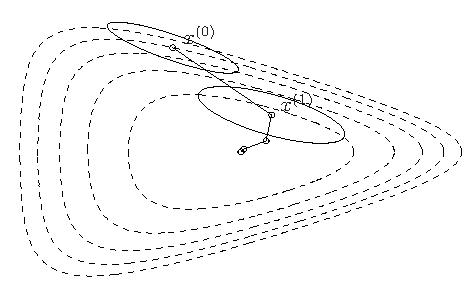
\includegraphics[width=.65\linewidth]{figures/ch09-fig19.pdf}
\caption*{图9.19\quad 对目标为（9.20）的 $\R^2$ 问题应用牛顿法，回溯参数为 $\alpha=0.1,\beta=0.7$。还显示前两个迭代点处的椭球 $\{x\mid\norm{x-x^{(k)}}_{\nabla^2f(x^{(k)})}\le1\}$。}
\end{figure}
\subsection{例子}
\subsubsection*{$\R^2$ 中的例子}
首先对测试函数（9.20）应用回溯线搜索牛顿法，参数 $\alpha=0.1,\beta=0.7$。图9.19显示牛顿迭代点，以及前两个迭代点 $k=0,1$ 的椭球
\[
\{x\mid\norm{x-x^{(k)}}_{\nabla^2f(x^{(k)})}\le1\}.
\]
方法有效，是因为这些椭球很好地近似下水平集的形状。

图9.20显示同一例子误差与迭代次数的关系，仅五次迭代就达到很高精度。二次收敛十分明显：最后一步把误差从约 $10^{-5}$ 降至 $10^{-10}$。

\subsubsection*{$\R^{100}$ 中的例子}
图9.21显示回溯与精确线搜索牛顿法在 $\R^{100}$ 问题上的收敛。目标具有（9.21）的形式，数据和初始点与图9.6相同。回溯线搜索曲线显示八次迭代即达很高精度。与 $\R^2$ 例子一样，第三次迭代后明显呈二次收敛。精确线搜索牛顿法仅比回溯少一次迭代，这也很典型：精确线搜索通常只对牛顿法收敛带来很小改进。图9.22显示步长。两个阻尼步之后，回溯线搜索所取均为完整步，即 $t=1$。

改变回溯参数 $\alpha,\beta$ 的实验表明，本例和其他例子中，它们对牛顿法性能影响很小。

% Source PDF page 507 (printed p. 493)
\begin{figure}[htbp]\centering
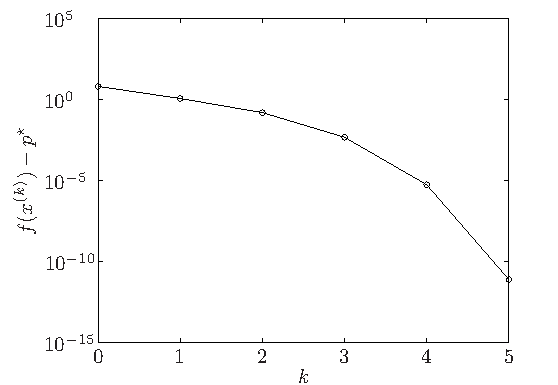
\includegraphics[width=.7\linewidth]{figures/ch09-fig20.pdf}
\caption*{图9.20\quad $\R^2$ 问题牛顿法的误差随迭代次数 $k$ 的变化。五次迭代即收敛到很高精度。}
\end{figure}
\begin{figure}[htbp]\centering
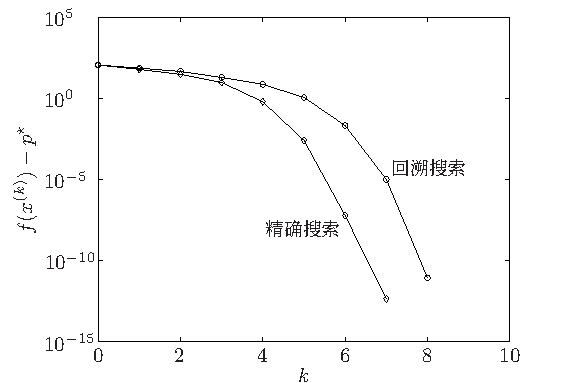
\includegraphics[width=.7\linewidth]{figures/ch09-fig21.pdf}
\caption*{图9.21\quad $\R^{100}$ 问题牛顿法的误差随迭代次数的变化。回溯参数为 $\alpha=0.01,\beta=0.5$。收敛也极快，七或八次迭代就有很高精度。精确线搜索仅比回溯快一次迭代。}
\end{figure}

% Source PDF page 508 (printed p. 494)
\begin{figure}[htbp]\centering
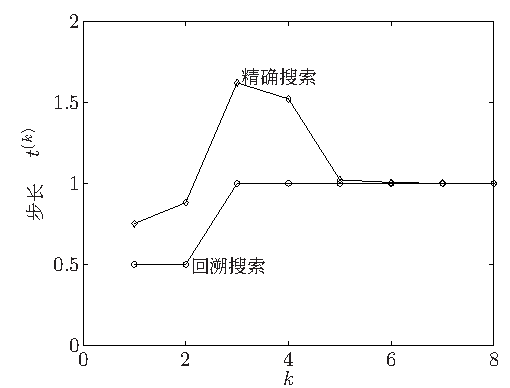
\includegraphics[width=.65\linewidth]{figures/ch09-fig22.pdf}
\caption*{图9.22\quad $\R^{100}$ 问题中，采用回溯和精确线搜索的牛顿法步长 $t$ 随迭代次数的变化。前两次迭代中，回溯线搜索各回溯一次；两次之后总选 $t=1$。}
\end{figure}
固定 $\alpha=0.01$，将 $\beta$ 在0.2至1之间变化，所需次数在8至12之间。固定 $\beta=0.5$，$\alpha$ 取0.005至0.5之间任意值时，所需次数均为8。因此多数实际实现采用较小 $\alpha$（如0.01）和较大 $\beta$（如0.5）的回溯线搜索。

\subsubsection*{$\R^{10000}$ 中的例子}
最后考虑一个更大的问题：
\[
\text{最小化}\quad
-\sum_{i=1}^n\log(1-x_i^2)-\sum_{i=1}^m\log(b_i-a_i^\T x),
\]
其中 $m=100000$、$n=10000$。数据 $a_i$ 是随机生成的稀疏向量。图9.23显示参数 $\alpha=0.01,\beta=0.5$ 的回溯线搜索牛顿法收敛。表现与前面的图很相似：约13次迭代的初始线性收敛阶段之后是二次收敛阶段，再用4或5次迭代就达很高精度。

\subsubsection*{牛顿法的仿射不变性}
牛顿法一个非常重要的特点是独立于线性或仿射坐标变换。设 $x^{(k)}$ 是对 $f:\R^n\to\R$ 应用牛顿法的第 $k$ 个迭代点。设 $T\in\R^{n\times n}$ 非奇异，定义 $\overline f(y)=f(Ty)$。若从 $y^{(0)}=T^{-1}x^{(0)}$ 出发，对 $\overline f$ 采用相同回溯参数的牛顿法，

% Source PDF page 509 (printed p. 495)
\begin{figure}[htbp]\centering
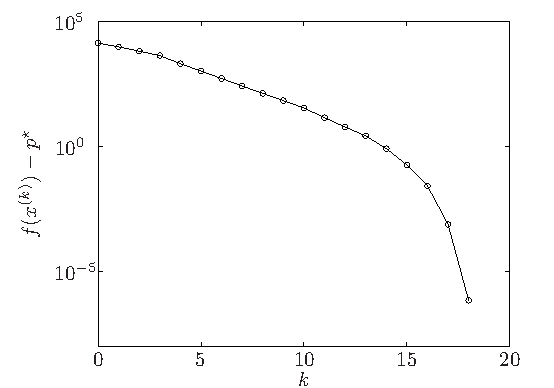
\includegraphics[width=.7\linewidth]{figures/ch09-fig23.pdf}
\caption*{图9.23\quad $\R^{10000}$ 问题的牛顿法误差随迭代次数的变化。采用 $\alpha=0.01,\beta=0.5$ 的回溯线搜索。即使这一大规模问题，牛顿法也仅需18次迭代就达很高精度。}
\end{figure}
则对所有 $k$，
\[
Ty^{(k)}=x^{(k)}.
\]
换言之，牛顿法相同：迭代点由同一个坐标变换联系。甚至停止准则也相同，因为 $\overline f$ 在 $y^{(k)}$ 的牛顿减量与 $f$ 在 $x^{(k)}$ 的相同。这与梯度法或最速下降法强烈受坐标变换影响形成鲜明对照。

例如，考虑（9.22）以参数 $\gamma$ 标记的问题族，$\gamma$ 影响下水平集条件数。图9.7和9.8中，当 $\gamma<0.05$ 或 $\gamma>20$，梯度法慢到无法使用。反之，对于 $10^{-10}$ 至 $10^{10}$ 间任意 $\gamma$，牛顿法（$\alpha=0.01,\beta=0.5$）都在九次迭代中求解此问题，而且精度高得多。

在采用有限精度运算的实际实现中，牛顿法并非完全独立于仿射坐标变换或下水平集条件数。不过，即使条件数高达 $10^{10}$，也不会对实际牛顿法实现造成不利影响；梯度法能容忍的条件数范围则小得多。坐标选择（或下水平集条件数）对梯度和最速下降法是首要问题，对牛顿法则是次要问题；它仅影响计算牛顿步所需的数值线性代数。

% Source PDF page 510 (printed p. 496)
\subsubsection*{小结}
牛顿法相比梯度与最速下降法，有几个突出的优点：
\begin{itemize}
\item 一般情况下收敛快，在 $x^\star$ 附近二次收敛。一旦进入二次收敛阶段，至多约六次迭代就能产生很高精度的解。
\item 仿射不变。对坐标选择或目标下水平集条件数不敏感。
\item 随问题规模增长表现良好。在 $\R^{10000}$ 问题上的表现与 $\R^{10}$ 相似，所需步数只适度增加。
\item 良好性能不依赖算法参数的选择。相比之下，最速下降法的范数选择对性能起关键作用。
\end{itemize}
牛顿法的主要缺点，是构造、存储Hessian以及计算牛顿步的成本；后者需要求解线性方程组。§9.7将说明，许多情况下可以利用问题结构，大幅降低牛顿步的计算成本。

另一选择是一类称为\emph{拟牛顿法}的无约束优化算法。它们形成搜索方向的计算量较小，但保留牛顿法的一些显著优点，例如在 $x^\star$ 附近快速收敛。由于许多书都介绍拟牛顿法，且它与本书主线关系不密切，本书不再讨论。
